\chapter{The International Linear Collider}
\label{ILC}
\begin{chapterabstract}
For answering the fundamental questions of mankind, it is necessary to understand the world in great detail.
In order to confirm theories in particle physics, or to disprove them, it is often important to be able to measure the qualities of particles or their interactions to several decimal places.
For measurements in high-energy particle colliders, such precisions can only be reached in linear lepton colliders.
The following sections will present a new design for such a collider on the precision frontier: the International Linear Collider (ILC). 
Its proposed layout, the possible construction sites, the detectors, and the physics motivation for such a capable accelerator will be explained.
\end{chapterabstract}
\newline

The International Linear Collider (ILC) is a proposed linear \positron\electron collider with a center-of-mass energy of \SI{250}{\GeV}, extendable to 350-\SI{500}{\GeV} and possibly even \SI{1}{\TeV}.
Its high luminosity and its state of the art technologies for the detectors and the machine will make the ILC an unprecedented precision machine, complementary to the currently existing high-energy physics accelerators, such as the Large Hadron Collider (LHC) at CERN.
The designs of the collider and the detector concepts are a result of over twenty years of research at over 300 science laboratories and universities all over the world~\cite{TDR1}.
The ILC project is therefore truly an international project.

\section{The ILC layout}
\label{ILC:layout}
The ILC was originally designed to collide electron and positron beams with a center-of-mass energy of \SI{500}{\GeV} in the first stage of operation.
The layout, as well as research results and physics motivations of this \SI{500}{\GeV} machine were summarized in great detail in the Technical Design Report (TDR) in 2013~\cite{TDR}.
Because of political developments and the request in 2017 to reduce the initial construction cost, the first stage collision energy was reduced to \SI{250}{\GeV}.
As it is in the nature of linear accelerators that the beam energy is linearly proportional to the accelerator length, the basic layout of the ILC as stated in the TDR is still the same for the new so-called ILC250.
However, the changes that were made to the layout are given in this section, together with an overview of the generation, preparation and collision of the particle beams in this linear collider concept.
%This is also the reason why the ILC has the possibility to upgrade the machine to higher energies later on.

\subsection{From beam generation to collision}
\label{ILC:layout:details}
\paragraph{Beam sources}
Figure~\ref{fig:ILC_Layout} shows the schematic layout of the ILC.
\begin{figure}
\centering
\includegraphics[width=0.8\textwidth]{Figures/ILC_layout_edited.png}
\caption[Schematic layout of the ILC]{Schematic layout of the ILC~\cite[based on p. 9]{TDR1}}
\label{fig:ILC_Layout}
\end{figure}
The electrons are produced by a GaAs photocathode in a DC electron gun~\cite[p. 13]{TDR32}.
By shining a circularly polarized laser on the electron beam, a beam polarization of at least \SI{80}{\percent} is achived, i.e. more than \SI{80}{\percent} of all electrons have the same handedness\footnote{For a left-handed particle, its spin and its momentum are antiparallel, pointing in opposite directions, and vice versa for a right-handed particle.}~\cite[p. 81]{TDR32}:
\begin{equation}
 P_e = \frac{N_L-N_R}{N_L+N_R} > 0.8
\end{equation}
The electrons from the electron source are captured and continue along the electron beam line.
The beam lines contain several sub-systems that prepare the beams for the main acceleration and the final collision.
One of the first sub-systems of the electron beam line is the initial bunching and pre-acceleration of the beam with normal-conducting RF cavities.
This is done using ``velocity bunching'', as explained in Section~\ref{AccPhysics:Bunching}.
Being pre-accelerated to \SI{76}{\MeV} in this step, the now `bunched' electron beams are accelerated to \SI{5}{\GeV} by a  superconducting booster linac~\cite[p. 81f]{TDR32}.\\
The positron source consists of an undulator and a conversion target~\cite[p. 90f]{TDR32}.
In an undulator, dipole magnets are placed in a line in such a way that their polarity alternates periodically (see Figure~\ref{fig:Undulator}).
For the creation of the positrons, the electron beam is used, which is guided through a \SI{231}{\meter} long helical undulator after being accelerated to the final beam energy of \SI{125}{\GeV}.
Using an undulator with a helical magnetic field causes the electrons to be deflected on a helical trajectory, and to emit synchrotron radiation photons that are circularly polarized\footnote{For circularly polarized light, the field vector of its electromagnetic wave rotates around the direction of propagation.}.
The high-energy photons are then converted in the \SI{7}{\milli\meter} thick titanium-alloy conversion target, where \positron \electron pairs are produced due to pair production.
As the pair production from circularly polarized photons yields longitudinally polarized \positron \electron pairs~\cite{Polarization}, the beam of the captured positrons will have a polarization of at least \SI{30}{\percent}~\cite[p. 14]{TDR32}.
The whole process leads to an effective positron yield of 1.5 positrons per original beam electron passing through the undulator~\cite{Ushakov}.
Due to the fact that the positrons were produced by using an already bunched electron beam, the positron beam is bunched as well. 
\begin{figure}
\centering
\includegraphics[width=0.45\textwidth]{Figures/Undulator_edited.png}
\caption[Schematic layout of an undulator]{Schematic of an electron beam traveling through an undulator with dipole magnets in alternating order~\cite[based on p. 41]{Wille}.}
\label{fig:Undulator}
\end{figure}
\paragraph{Damping rings}
Since the electrons and positrons still have a large emittance from when they originated from their sources, their momentum and beam sizes have to be condensed.
This is done in the damping rings, which have a circumference of \SI{3.2}{\kilo\meter}~\cite[p. 14]{TDR32}.
A layout of the ILC damping rings is shown in Figure~\ref{fig:DR}.
As discussed before, the beams will emit synchrotron radiation when they are deflected in a magnetic field.
This is desired in the damping rings in order to ``cool'' the beams, i.e. to reduce their momenta due to the emission of photons.
The emission of synchrotron radiation happens in the curved sections of the damping rings, but also in the straight sections by the use of wigglers.
Wigglers are similar to undulators, but use fewer magnet pairs and higher magnetic fields.
Charged particles are therefore deflected more in wigglers.
Since the synchrotron radiation photons are emitted tangentially to the beam particle's path, the particle's momentum in the forward direction is reduced.
By accelerating the beams in RF cavities in the straight sections, the beam momentum in the z-direction is increased.
Overall, the momentum in the desired direction rises, whilst the momentum spread shrinks.
\begin{figure}[h]
\centering
\includegraphics[width=0.4\textwidth]{Figures/DR.png}
\caption[Damping ring layout]{Schematic layout of the ILC damping rings.
Next to the injection and extraction system, there are wigglers and RF cavities for the emittance reduction, as well as a chicane for circumference adjustments, and a so-called phase trombone for accommodating changes in the RF phase~\cite[p. 15]{TDR32}.}
\label{fig:DR}
\end{figure}
\\This is, however, not the only effect of damping rings.
As shown in Section~\ref{AccPhysics:Bunching}, the orbit of charged particles in an external magnetic field depends on their momenta.
In the bends, off-momentum particles travel on an orbit with a different radius than particles with the ideal momentum.
Entering the straight sections from suboptimal orbits causes orbit distortions and aberrations in the straight sections, which again causes a rise in the beam emittance.
To counteract this effect, a chicane (see Chapter~\ref{AccPhysics:Bunching}) is needed for adjusting the circumference.
An additional phase trombone system, which consists of sets of alternating quadrupoles, regulates the orbit aberrations due to changes in the RF phase.
Because of the design choice of having a pulse repetition rate of \SI{5}{\hertz}, the beams are stored for \SI{200}{\milli\second} in the damping rings, performing about \num{18000} turns.
After this amount of turns, an equilibrium emittance is reached, and the high quality beam with small beam emittance is extracted and continues along the beam lines.

\paragraph{Bunch compressors}
After passing the damping rings, the electron and positron beams are compressed in bunch length by a two-stage compressor system, using ``magnetic compression''.
Here, the bunch length is reduced from several millimeters to \SI{300}{\micro\meter}.
In both compressor systems, RF cavities are used together with wigglers, which compact the beam momentum by exploiting the momentum spread within the beam bunch.
As discussed in Section~\ref{AccPhysics:Bunching}, the RF frequency and the timing is chosen such that the bunch tail experiences an accelerating phase in the RF cavity, whilst the bunch head experiences a decelerating phase.
The low-momentum particles of the bunch head will therefore be deflected more in the wiggler, whilst the high-momentum particles of the tail are deflected less.
At the end of the compressor system, the particles of the bunch tail and head will have gotten closer, leading to a shortened beam bunch. 
The usage of two separate systems relaxes the requirements a single system would need to fulfill, and allows more flexibility in the operation, e.g. to reduce the beam length below \SI{300}{\micro\meter}~\cite[p. 124]{TDR32}.

\begin{figure}[h!]
\centering
\includegraphics[width=0.4\textwidth]{Figures/Cavity_Gradient.png}
\caption[XFEL cavity gradient]{Maximum and usable gradient distribution of the final European XFEL cavities.
The number of cavities showing a certain gradient is displayed as the bar chart.
The so-called usable gradient is the effective gradient a cavity reaches under strict requirements, such as achieving the operational specification for the quality factor.
The yield, which is shown as the line graphs, is defined as the fraction of cavities which have a gradient higher than the specified value on the x-axis~\cite[p. 18]{XFEL_Cavities}.}
\label{fig:XFEL_cav}
\end{figure}
\paragraph{Main linacs}
Subsequent to bunch compressors, the bunches are injected into the main linear accelerator structures (main linacs).
The two main linacs are designed to accelerate the beams to the final beam energy of \SI{125}{\GeV}, leading to a center-of-mass energy of \SI{250}{\GeV}.
They have a length of \SI{5}{\kilo\meter} each, and use \SI{1.3}{\giga\hertz} superconducting RF cavities with an average accelerating gradient of \SI{31.5}{\mega\volt\per\meter}~\cite{Walker}.
A picture of one of these cavities is shown in Figure~\ref{fig:Tesla_Cavity}. 
Since cavities of the same design are already in use for the European XFEL (X-Ray Free-Electron Laser) at Deutsches Elektronen-Synchrotron (DESY) in Hamburg, their high performance has already been demonstrated~\cite{XFEL}.
The gradient distribution of the cavities used at the European XFEL is shown in Figure~\ref{fig:XFEL_cav}.
The average of the maximum gradient reachable per cavity module is about \SI{35}{\mega\volt\per\meter}, which is higher than the ILC requirements.
This is especially remarkable, as the cavity specifications for the European XFEL are lower than for the ILC.
Another key point is that the production of the cavities is an industrialized process.
The high gradients are therefore not demonstrated in a laboratory environment only, but the gradients are also achieved in a more automated procedure.

\begin{figure}[h!]
\centering
\includegraphics[width=0.6\textwidth]{Figures/BDS.png}
\caption[Layout of the Beam Delivery System]{Schematic layout of the Beam Delivery System (BDS) for the electron beam line.
After the main linac, the BDS for the electron beam line reaches from about Z = -2.2\,km to the Interaction Point (IP) at Z = 0.
The vertical colored lines along the beam line represent the magnets and other devices of the various sub-systems.
Next to diagnostic devices, such as the polarimeter and the energy spectrometer, there are collimation systems to focus and to prepare the beam for the collision at the IP.
The primary dump at Z = 250\,m is the electron beam dump~\cite[p. 135]{TDR32}.}
\label{fig:BDS}
\end{figure}
\paragraph{Beam Delivery System}
The Beam Delivery System (BDS), which has an overall length of about \SI{4.4}{\kilo\meter}, transports the bunches from the linacs to the Interaction Point (IP).
In the BDS, the beams are focused to nanometer size by the Final-Focus (FF) system, which is a crucial part of the ILC program.
Only with nanometer-sized bunches can the ILC can reach luminosities comparable to or beyond the Large Hadron Collider (LHC) at CERN, since the total production cross section for \positron \electron colliders is several orders of magnitude smaller than for proton-proton colliders, such as the LHC, at their respective collision energies (see Figure~\ref{fig:Cross_sections}).
To demonstrate the feasibility of nanometer-scale beams, a test facility was built that is a small scale prototype of the FF system for the ILC: the Accelerator Test Facility (ATF2), which will be presented in more detail in Section~\ref{ATF2}.
The BDS system not only contains the FF system, but also various feedback diagnostics and beam-halo collimators for removing the halo of particles around the beam core in order to reduce the beam background at the IP. 
The sub-system layout for the sophisticated BDS is shown in Figure~\ref{fig:BDS}.
Additionally, shielding systems are installed at various locations along the BDS line, again in order to keep the background level at the IP as low as possible.
Chapter~\ref{BDS_Muons} will talk about muon shielding options that are considered for the ILC.

\paragraph{Beam collision}
After the Final-Focus system, the beams are then finally brought into collision with a crossing angle of \SI{14}{\milli\radian} at the IP.\cite[p. 9-10]{TDR1}
With so-called crab cavities, the bunches are rotated horizontally so that effective head-on collisions are possible.
This is illustrated in Figure~\ref{fig:Crab_crossing}.
The crab cavities are also superconducting RF cavities, but designed for a RF frequency of \SI{3.9}{\giga\hertz} and an accelerating gradient of \SI{5}{\mega\volt\per\meter}~\cite[p. 154]{TDR32}.
The RF phase is modeled in such a way that only the head and the tail of the beam bunch experience acceleration, but in opposite directions.
The voltage needed to rotate a bunch with energy $E_{bunch}$ can be calculated as follows~\cite{Crab_cavities}:
\begin{equation}
 V_{crab}=\frac{cE_{bunch}\theta_C}{2\omega R}
\end{equation}
$\theta_C$ is the crossing angle as before, $\omega$ is the RF frequency of the crab cavity, and $R$ is the ratio of the bunch displacement at the IP to its divergence, i.e. the ratio of the spatial shift at the IP to the increase in the beam size.
With all other quantities fixed, only $R$ can be increased in order to reduce the required voltage.
Therefore, the crab cavities are positioned at locations where this ratio $R$ between the spatial shift and the beam size increase is calculated to be large.
For the ILC, it was calculated that the crab cavities should be located \SI{13.4}{\meter} up- and downstream of the IP~\cite[p. 154]{TDR32}.
\begin{figure}
\centering
\includegraphics[width=0.4\textwidth]{Figures/Crab_crossing.png}
\caption[Schematic of a beam crossing with crab cavities]{Schematic of a beam crossing with crab cavities. In a crossing with crossing angle $\theta_C$, head-on collisions are only possible with crab cavities that rotate the beam in the horizontal plane.}
\label{fig:Crab_crossing}
\end{figure}

\paragraph{Beam parameters}
Table~\ref{tab:ILC_parameters} shows the beam parameters for the baseline design at \SI{250}{\GeV} center-of-mass energy, and for the energy and the luminosity upgrade stages.
%\multicolumn{1}{>{\centering}p{1.5cm}}{\textbf{Baseline 500}} & \multicolumn{1}{>{\centering}p{1.5cm}}{\textbf{Lumi Upgrade}} & \multicolumn{1}{>{\centering}p{1.5cm}}{\textbf{TeV Upgrade}} & {\centering\textbf{LHC 25ns}} \\ 
\begin{table}[h]
\caption{Beam parameters for different phases in the ILC operation scenario (ILC250, ILC500, Luminosity Upgrade, TeV Upgrade)~\cites[p. 11]{TDR1}{CR-0016} in comparison to LHC Run 2 beam parameters~\cites[p. 3ff]{LHC_TDR}{LHC_Parameters}.}
\label{tab:ILC_parameters}
\centering
\begin{tabularx}{0.99\textwidth}{lll|rrrrg}
\hline\hline
& && \multicolumn{1}{>{\centering}p{1.5cm}}{\textbf{ILC250}} & \multicolumn{1}{>{\centering}p{1.5cm}}{\textbf{ILC500}} & \multicolumn{1}{>{\centering}p{1.5cm}}{\textbf{Lumi Up}} & \multicolumn{1}{>{\centering}p{1.5cm}}{\textbf{TeV\\Up}} & \multicolumn{1}{>{\centering}p{1.5cm}}{\textbf{LHC 25ns}}\\
\hline
\cline{1-8}
\hline
E$_{CM}$  &{\small Center-of-mass energy}&{\small(\si{\GeV})}& 250 & 500  & 500  & \num{1000} & \num{14000}\\
n$_b$ &{\small Number of bunches}&& \num{1312} & \num{1312} & \num{2625} & \num{2450} & \num{2808} \\
$f_{rep}$ &{\small Pulse repetition rate}&{\small(\si{\hertz})} & 5 & 5  & 5   & 5 & \num{11245}\\
$\Delta t_b$ &{\small Bunch seperation}&{\small(\si{\nano\second})} & 554 & 554  & 366   & 366 & 25\\
N &{\small Bunch population}&& 2.0$\cdot10^{10}$ & 2.0$\cdot10^{10}$  & 2.0$\cdot10^{10}$  & 1.74$\cdot10^{10}$ & 11.5$\cdot10^{10}$\\
q$_b$ &{\small Bunch charge}&{\small(\si{\nano\coulomb})}  & 3.2 & 3.2  & 3.2  &  2.7 & 18.4  \\
$\sigma_x^*$ &{\small Horiz. beam size at IP}&{\small(\si{\nano\metre})} & 515.5 & 474  & 474  &  481 & \num{16700}\\
$\sigma_y^*$ &{\small Vert. beam size at IP}&{\small(\si{\nano\metre})} & 7.7 & 5.9 &  5.9  &  2.8 & \num{16700}\\
$\sigma_z$ &{\small Longit. beam size}&{\small(\si{\milli\metre})} & 0.3 & 0.3  &  0.3  &  0.25 & 0.755\\
L &{\small Luminosity}&{\small(\si{\per\centi\metre\squared\per\second})} & 1.35$\cdot10^{34}$ & 1.8$\cdot10^{34}$ & 3.6$\cdot10^{34}$ &3.6$\cdot10^{34}$ & 1.0$\cdot10^{34}$\\
\hline\hline
\end{tabularx}
\end{table}
For all ILC running scenarios, the beam sizes are several orders of magnitude smaller than for the LHC Run 2, which is the reason for the comparable luminosities as mentioned above.
Despite the number of bunches per pulse and the bunch population being smaller, the LHC luminosity can be exceeded.
It is striking that the beam sizes in the horizontal and vertical plane are symmetric for the LHC, whereas they are different for the ILC.
This is a design choice, reducing the effect of beamstrahlung whilst enhancing the luminosity.
As shown in Equation~\ref{eq:pair_number}, the number of background particles from beamstrahlung is inversely proportional to the sum of the beam sizes, $\sigma_x+\sigma_y$.
At the same time, the luminosity is inversely proportional to the product of the beam sizes, $\sigma_x\cdot\sigma_y$, as shown in Equation~\ref{eq:luminosity} in Chapter~\ref{AccPhysics:Linear-Circular}.
By choosing the beam sizes to be $\sigma_x\gg\sigma_y$, the product is small leading to large luminosities, while the sum is large leading to a diminished background rate.

\paragraph{Interaction region and beam dumps}
The Interaction Region (IR) houses the two detectors for the ILC: the Silicon Detector (\sid) and the International Large Detector (ILD), which are in a so-called ``push-pull'' system.
The detectors and the push-pull system are explained in more detail in Section~\ref{ILC:detectors}.\\
Finally, after collision the spent beams are guided through the extraction line towards the main beam dumps, where they are dumped.
The current designs for the main beam dumps are based on a water tank, using high-pressure water with velocity flow systems.
Since the water tanks are designed to be sufficient for all energy and luminosity stages, they are supposed to withhold a particle beam with a beam power of \SI{14}{\mega\watt} for the \SI{1}{\TeV} operation~\cite[p. 18]{TDR32}.
This leads to high irradiation of the beam dump surrounding and dangerous conditions for maintenance staff.
In Chapter~\ref{BeamDumps}, which talks about the simulation of the main beam dumps done for this thesis, more details are given for the current beam dump designs.

\subsection{Staging}
\label{ILC:layout:staging}
As mentioned above, the panel of the International Committee for Future Accelerators (ICFA) officially decided in 2017 to reduce the center-of-mass energy of the first ILC stage to \SI{250}{\GeV}, in order to reduce the total costs of the ILC project.
ICFA's official statement declares that the ``[...] International Linear Collider (ILC) operating at 250 GeV center-of-mass energy will provide excellent science from precision studies of the Higgs boson.
Therefore, ICFA considers the ILC a key science project complementary to the LHC and its upgrade.
ICFA welcomes the efforts by the Linear Collider Collaboration on cost reductions for the ILC [...]''~\cite{ICFA_Statement}.\\
The total costs for realizing the ILC includes the manpower, the costs for the construction of the so-called conventional facilities, such as the underground tunnels and the surface buildings, and the costs for the production and assembling of the accelerator and detector components.
When breaking the total costs down into the subsystems, then the conventional facilities together with the production of the RF modules for the main linacs make up almost \SI{75}{\percent} of the total costs~\cite[p. 20f]{TDR1}.
These estimations are based on cost inquiries with several industrial companies, as well as on experiences collected at other accelerator projects, such as the European XFEL which uses the same design for the RF cavities as planned for the ILC.\\
Regarding the ILC layout, several options are under discussion which are shown in Figure~\ref{fig:Staging}.
These options would yield a cost reduction of up to \SI{34}{\percent}~\cite{Cost_reduction}, resulting in about \SI{66}{\percent} of the initial costs for the \SI{500}{\GeV} machine by reducing the length of the tunnel (options A, B, and C), or by additionally reducing the number of RF cavities (options A', B' and C').
In options A', B', and C', the RF cavities are planned to have a larger accelerating gradient so that a smaller number of cavities would still lead to the same beam energy as for options A, B, and C.
Overall, option A' foresees the shortest possible tunnel for \SI{250}{\GeV} and the smallest number of cavities, and therefore results in the highest cost reduction.\\
As explained before, the costs for the tunnel and the accelerating structures represent indeed the largest fraction of the total costs, and will be reduced by the staging options.
However, the other parts of the accelerator and the surface buildings will not change by the staging scenarios but form basic costs because of which the maximum cost reduction cannot exceed \SI{34}{\percent}.
Therefore, it has to be considered whether the cost cutback of option A' outweighs all other options with a tunnel length suitable for an energy upgrade.
An extended tunnel would give a positive sign to the ILC community that an energy upgrade is definitely foreseen for the future.
\\Figure~\ref{fig:ILC_runningtime} shows two possible running scenarios for the staged ILC.
In both cases, the ILC will have energy and luminosity upgrades, so that it will reach the same integrated luminosity over a different amount of time.
On the left hand side, the plot shows an expected operation time of 15 years for the ILC250 with a luminosity upgrade at the midway-point.
As shown in Equation~\ref{eq:luminosity}, the luminosity of a particle collider is directly proportional to the number of bunches colliding in every beam pulse.
Hence, by increasing the number of bunches by a factor of two, the luminosity for the luminosity upgrade stage is doubled.
After an energy upgrade by extending the main linacs, the operation at \SI{500}{\GeV} and a short run at \SI{350}{\GeV} for dedicated measurements of the top quark qualities would be possible.
The overall operation time would stretch out to 26 years.\\
For the second scenario on the right hand side of Figure~\ref{fig:ILC_runningtime}, it was assumed that the beam parameters are changed in such a way that the beam is more strongly focused at the IP and therefore that the instantaneous luminosity is enhanced.
This shortens the operation time of the ILC250 stage to 11 years, and the overall run time to 22 years, whilst still achieving the same integrated luminosity~\cite[p. 7]{PhysicsCase}.
\begin{figure}
\centering
\includegraphics[width=0.9\textwidth]{Figures/Staging.png}
\caption[Different layouts for the ILC250 stage]{Different layouts for the ILC250 stage.
The original layout has foreseen a tunnel fitting linacs for \SI{250}{\GeV} beam acceleration, which would lead to a center-of-mass energy of \SI{500}{\GeV}.
For the new stage, the linacs are reduced in length.
The discussions about the layout involves also the length of the tunnel.
Option B and C would foresee longer tunnels that would facilitate a later energy upgrade to 350 or \SI{500}{\GeV}.\\
Options A', B' and C' correspond to options A, B and C regarding the tunnel length, but they assume RF cavities with a gradient of \SI{35}{\mega\volt\per\meter} instead of \SI{31.5}{\mega\volt\per\meter} in order to reduce the number of cavities needed~\cite[p. 19]{Staging}.}
\label{fig:Staging}
\end{figure}
\begin{figure}[htbp]
\centering
\includegraphics[width=0.98\textwidth]{Figures/ILC_runningtime.png}
\caption[ILC run plan]{Two possible ILC run plans for the staged ILC~\cite[p. 8]{PhysicsCase}.}
\label{fig:ILC_runningtime}
\end{figure}

\section{Possible site}
Out of originally more than ten potential ILC sites in Japan, the Kitakami mountains in the Tohuku Prefecture were chosen as the preferred site for the ILC~\cite{Site}.
This decision was made in August 2013 after a detailed study of all site specific factors, like the geological conditions, the infrastructure, and the impact on the environment and the economy.
Measurements of the Kitakami mountains have shown that it consists mostly of granite rock with the best qualities for the ILC, with respect to vibration and rock stress.
As can be seen in Figure~\ref{fig:ILC_Site}, the closest city (with about 120,000 citizens) would be Ichinoseki.
Morioka and Sendai are the biggest cities close to the candidate site, with Tokyo being about \SI{430}{\kilo\meter} away.
Although being in the north of Japan, the travel time from Tokyo is only about three hours by Shinkansen, Japan's high-speed bullet train, and the proximity to the coast line allows the transportation of construction, machine, and detector parts by ship.
Additionally, there are local airports in both, Morioka and Sendai, presenting further options for traveling and the transportation of construction materials.
\label{ILC:site}
\begin{figure}[h]
\centering
\includegraphics[width=0.6\textwidth]{Figures/ILC-site.png}
\caption[Possible site for the ILC]{The possible site for the ILC is the Kitakami mountains in the Tohuku prefecture.\cite{Kitakami}}
\label{fig:ILC_Site}
\end{figure}

\section{Physics motivation}
\label{ILC:physicsmotivation}
After having shown that the ILC as a linear lepton collider is designed to be a state-of-the-art precision machine, this section will present its physics goals.
With the LHC as a machine at the energy frontier, the ILC will be a complementary collider aiming rather for much needed precision than for searching for new particles at high energies.
The ILC therefore intends to find new particles and new physics through highest precision measurements.
It is often called the future Higgs factory which will measure the qualities of the Higgs boson with much higher precision than has been done so far.
Additionally, the different stages of the ILC will also measure the top quark qualities, and will have access to Beyond Standard Model (BSM) physics.
Since the first ILC stage will run at a center-of-mass energy of \SI{250}{\GeV}, this section will focus more on the measurements of the Higgs boson than of the top quark and the BSM physics.
 
\subsection{How to get there}
To reach the precision the ILC promises, it must achieve four different objectives.
These objectives are all linked so that one is dependent on the others.
In the following section, these four objectives of the ILC are explained in comparison to the LHC.

\paragraph{Minimal background}
Due to leptons in the initial state, there will be one physics process per colliding lepton pair.
Leptons are elementary and not composite particles like the proton, therefore there are no underlying events which arise from other partons of the composite particle.
The energy range of the final state particles is restricted, since the initial energy of the colliding beams can be set precisely and only point-like particles collide.
By adjusting the center-of-mass energy of the collision and running threshold scans at the mass of the particle of interest, the rate of the desired process can be increased.
This is only possible at lepton colliders.
\\Beam polarization contributes to the small background levels as well, since the polarization can be set in such a way that weak interactions are either enhanced or suppressed.
As the weak interaction acts only on left-handed fermions, the polarization (or handedness) of the beam particles has an effect on the processes that can occur.
This effect can be seen directly by looking at the two possible production modes at an \positron\electron collider (see also Chapter~\ref{Production_modes}):
direct \positron\electron annihilation, and \positron\electron scattering.
In the SM annihilation process, the electron and positron have to be of opposite handedness due to the nature of weak interactions.
The annihilation cross-section can therefore be enhanced by polarizing the beams to have opposite polarization.
For the \positron\electron scattering process, the handedness of the final state particles is dependent on the handedness of the incoming particles.
By setting different polarization combinations, the properties of the final state particles, the interactions, and the couplings can be studied. %Check out PhD Thesis of Annika Vauth, p.10-12
Therefore, depending on the physics process of interest, the polarization can enhance the signal whilst suppressing the background. 
\\Figure~\ref{fig:Cleanliness} shows two event displays of a Higgs event at the LHC and the ILC in comparison.
Due to the nature of composite particles, event displays at the LHC are dominated by underlying events and pileup events.
At the ILC, the event displays are clean, and the tracks from the final state particles of the physics event can be distinguished easily.
\begin{figure}
\centering
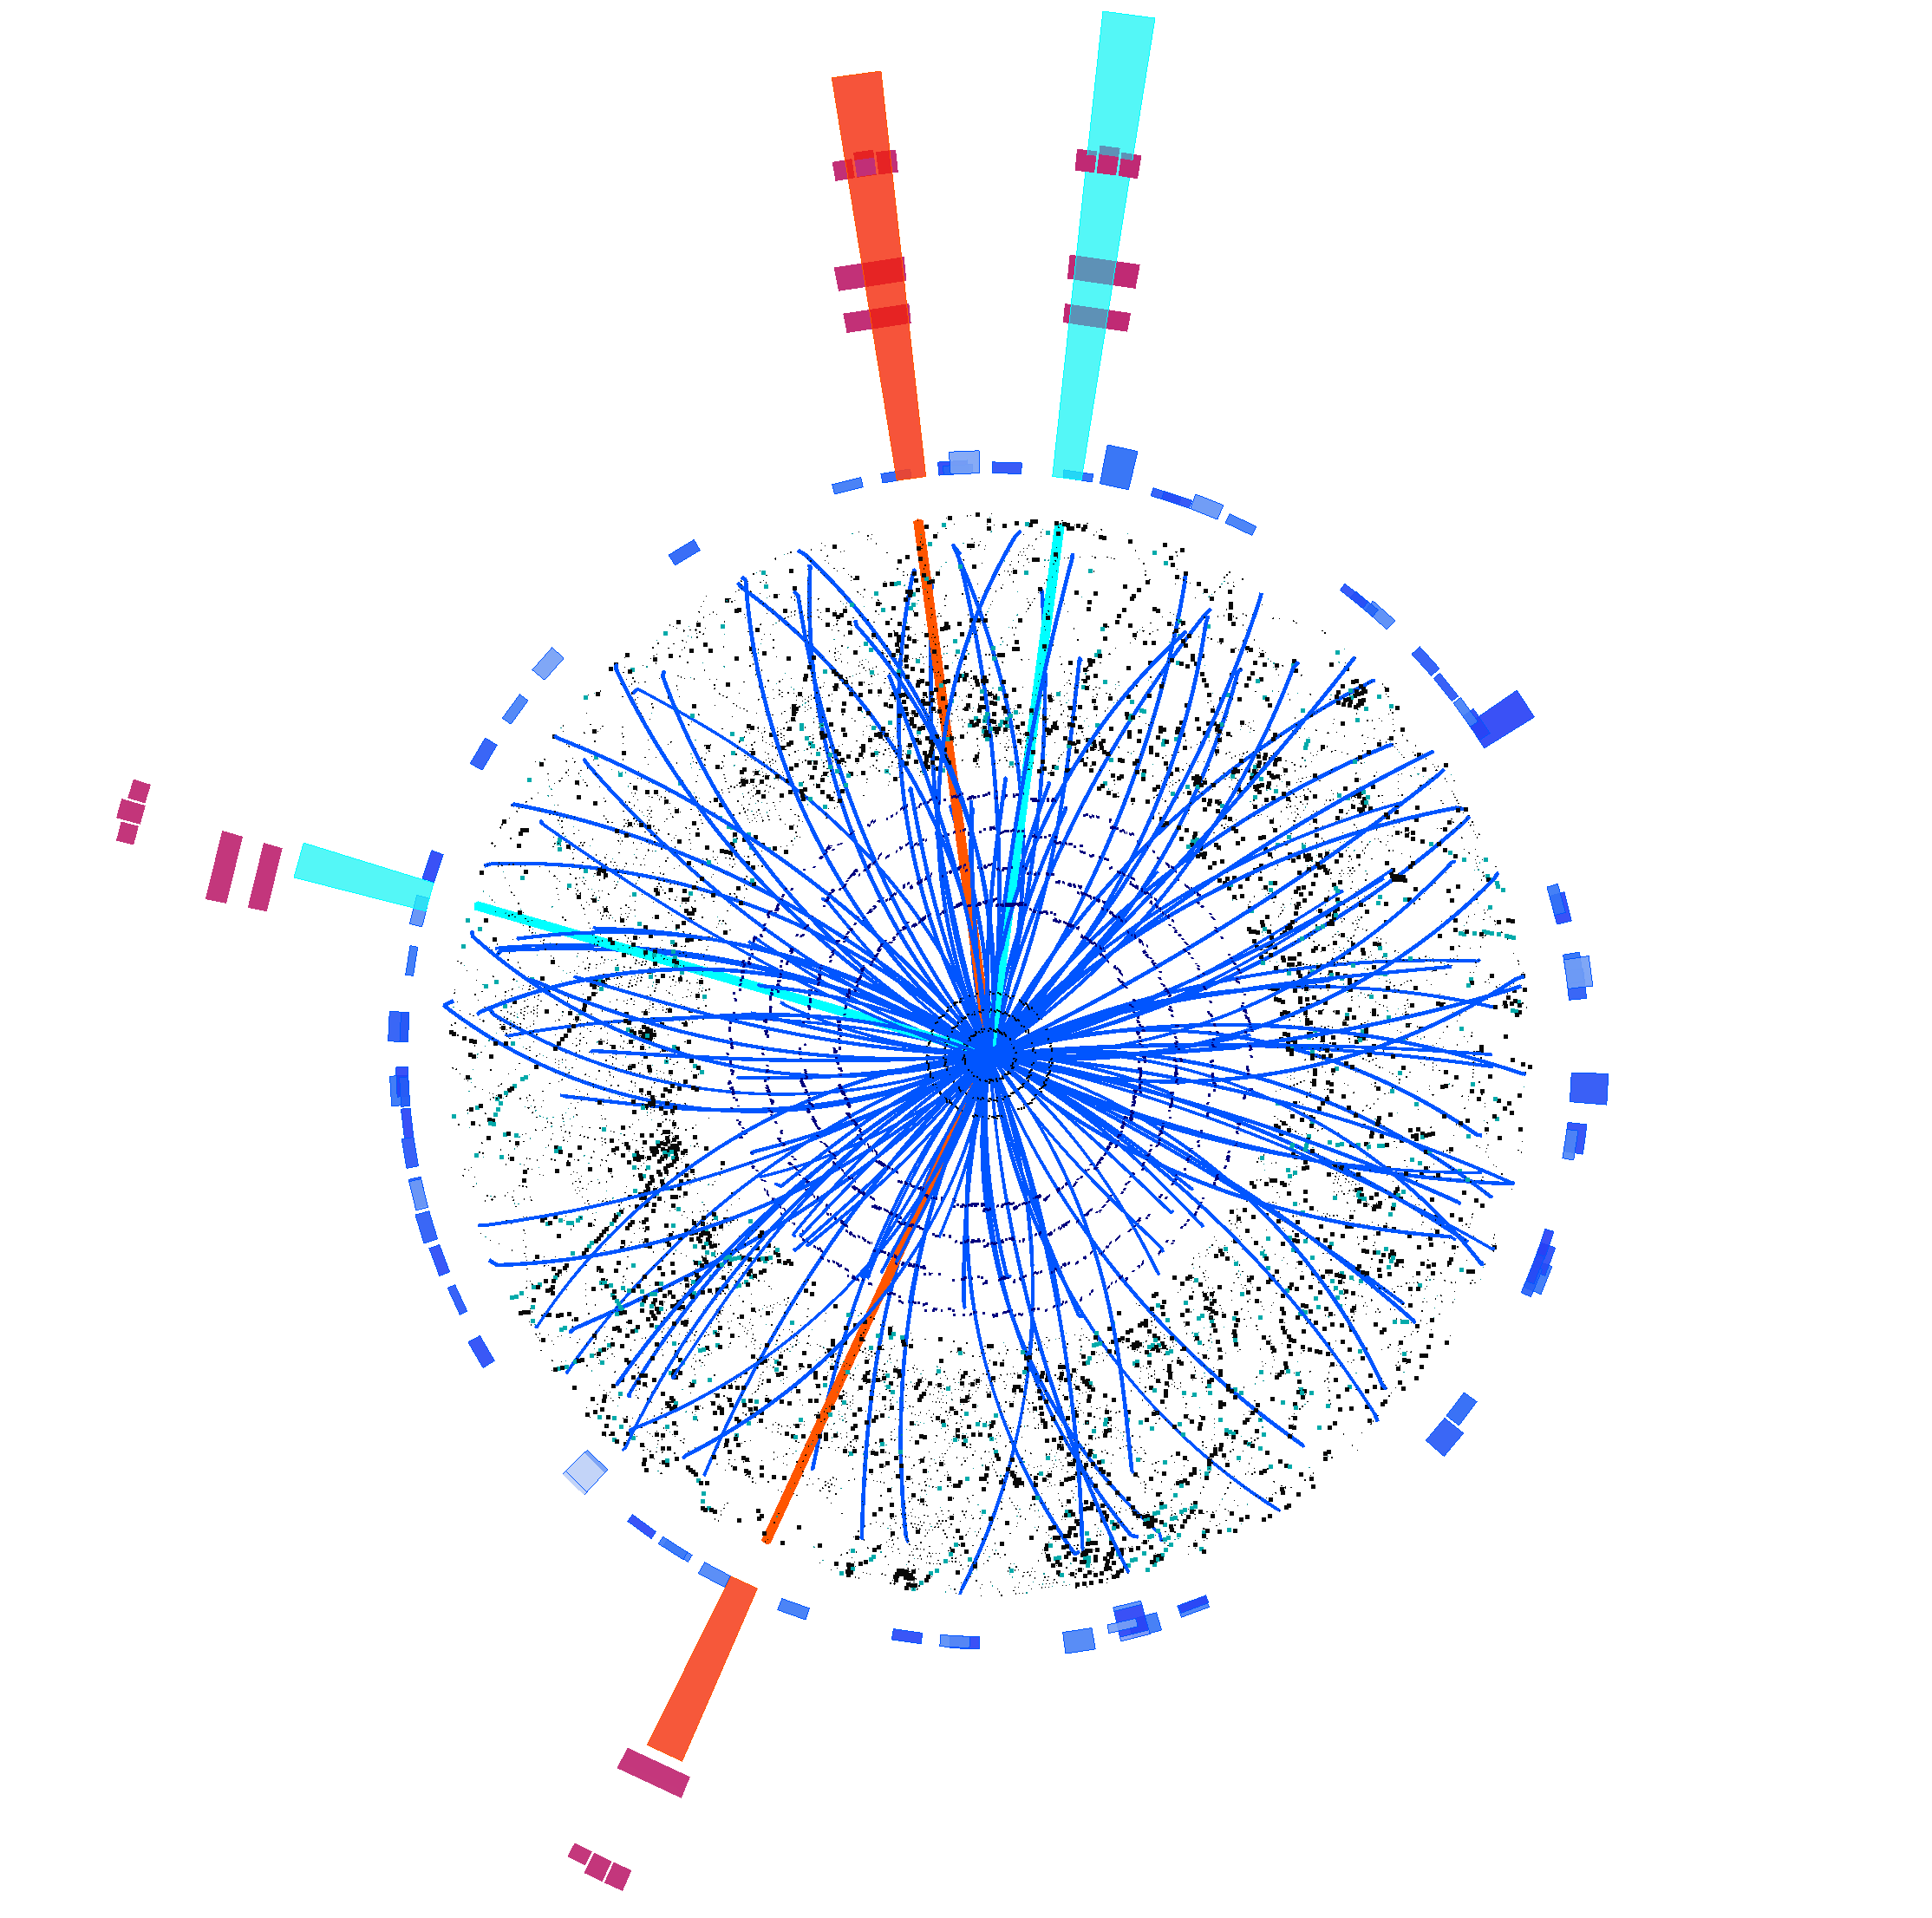
\includegraphics[width=0.3\textwidth]{Figures/ATLAS_event_display.png}
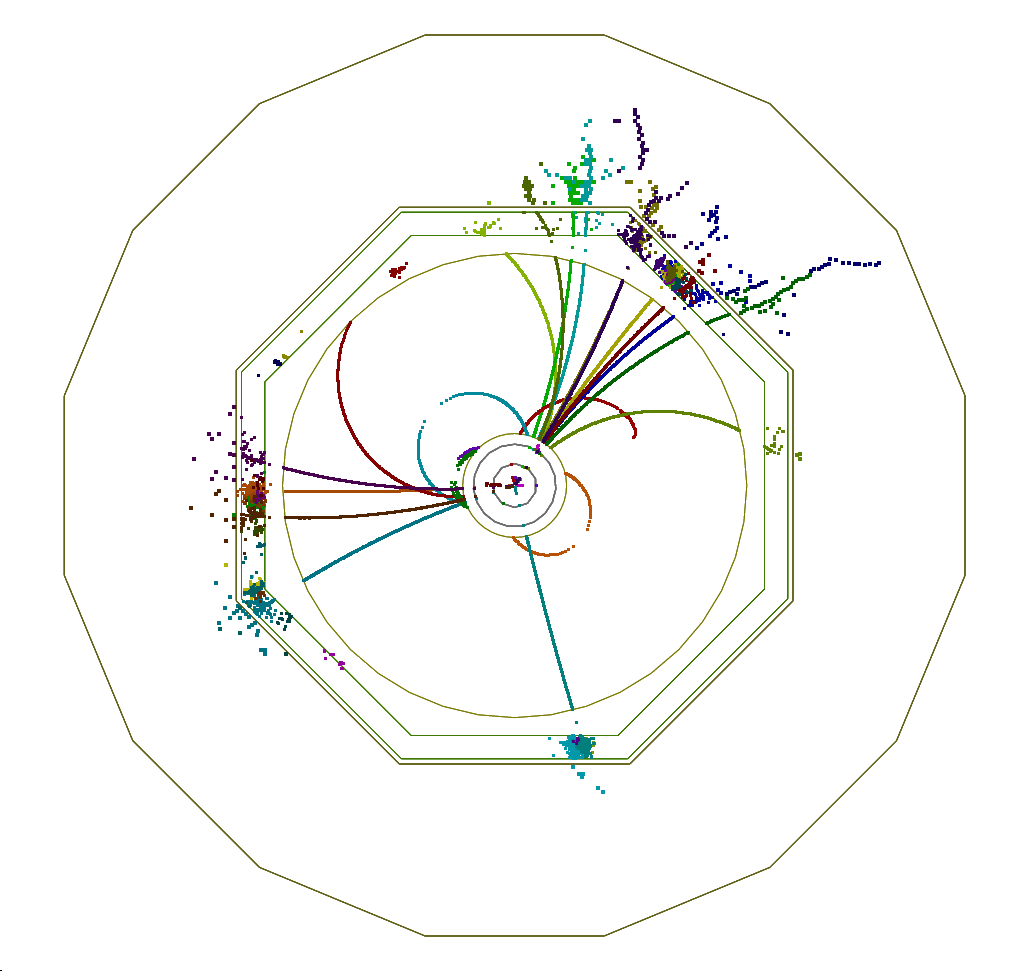
\includegraphics[width=0.3\textwidth]{Figures/ILD_event_display.png}
\caption[Clean environment at the ILC]{Comparison of the event displays of a Higgs event at the  LHC and at the ILC.
The left figure shows an event of a Higgs boson decaying to two \positron\electron pairs at the LHC~\cite{ATLAS_event_display}.
On the right, an event display of a Zh$\rightarrow$\positron\electron h event at the ILC is shown~\cite{ILD_event_display}.
\\At the LHC, underlying events and pileup events populate the detector, whilst at the ILC the hits are mainly from the final state particles of the physics interaction of interest.
}
\label{fig:Cleanliness}
\end{figure}

\paragraph{Democratic particle cross sections}
Because the elementary coupling of Z bosons and photons is of the same order for all quarks and leptons, the \positron\electron annihilation produces pairs of all species at similar rates.
In addition, the ILC will record all events without triggers.
This means that no process will be rejected, and the complete readout of all events measured with the detectors will be stored for later analysis.
This is only possible because the total number of detector hits from background events is small.
Small background levels therefore imply small detector occupancies.

\paragraph{Small uncertainties}
The initial state of all events is precisely known, both in terms of the particles undergoing the interactions and also the energies involved in the initial states.
Additionally, there are only events with couplings to electroweak interactions, so that PDF uncertainties and systematic uncertainties due to QCD corrections are omitted.
\\The small uncertainties enhance theoretical and experimental precisions at \positron\electron colliders.

\paragraph{Complete knowledge}
Because of the small background and the possibility to record and store the complete detector readouts, processes can be reconstructed in completeness without theoretical assumptions.
The quark and lepton momenta can therefore be determined by kinematic fits.
Studies of the spin-dependence of the production and decay processes are also possible.\\
Due to the high energy resolution and the fact that the initial particle energies are precisely known, particles with small mass differences are distinguishable, i.e. peaks in mass spectra that are close together are more likely to be separable.
That means that new particles might indeed be found at the ILC.\\
Additionally, c-tagging will be a possible tool for physics analyses, and will improve many physics studies at the ILC.
The life time of a charm quark (c) before it hadronizes is around \SI{80}{\micro\meter}, which is a perfect way to identify that a charm quark was involved in the event.
Since the distance between the primary and the secondary vertex can only be measured by a vertex detector with micrometer resolution, c-tagging is in general very difficult.
However, it will be possible at the ILC, because the detector concepts foresee such a resolution, and the nanometer-sized beam allows the inner vertex detector radius to be very close to the interaction point.
%only approximately \SI{10}{\milli\meter}. 
%charm hadron lifetime: 80microns, bottom hadron lifetime: 400microns

\subsection{ILC as a Higgs factory}
The ILC250 stage will be a so-called Higgs factory, tuned to a center-of-mass energy of \SI{250}{\GeV}, where the cross section $\sigma$ for Higgs production is at its maximum.
Due to the large luminosity and the capability for precision measurements, as has been shown in the section above, the individual Higgs boson qualities can be measured to a percent accuracy in a completely model independent way.
These Higgs boson properties include the Higgs mass, its couplings to Standard Model particles, as well as its total decay width.
In contrast, for the LHC experiments, global fits to all Higgs signals together with theoretical assumptions of its decay width is the only way to gain the Higgs couplings.
\\After a brief overview of the Higgs production modes and the determination of the Higgs properties at the ILC, it will be shown how the unprecedented precisions are achievable at the ILC.

\subsubsection{The Higgs production modes at an \positron\electron collider}
There are three main production modes for Higgs bosons at an \positron\electron collider, such as the ILC.
As can be seen in Figure~\ref{fig:HiggsProduction}, the largest contribution to the overall production cross section is the Higgsstrahlung process, where a Higgs boson is produced in association with a Z boson ($e^+e^-\rightarrow Zh$).
In vector boson fusion (VBF) processes, like the WW fusion and the ZZ fusion, the fusion of two bosons produces a Higgs boson and a pair of leptons.
For the WW fusion, an electron-neutrino and its anti-neutrino are produced ($e^+e^-\rightarrow \nu\bar{\nu} h$), whilst for the ZZ fusion it is an electron and a positron ($e^+e^-\rightarrow e^+e^-h$).
The production cross sections for these processes as a function of the center-of-mass energy behave quite differently:
The dominant process at energies between 200 and \SI{450}{\GeV} is the Higgsstrahlung process, replaced by the WW fusion process above \SI{450}{\GeV}.
The ZZ fusion cross section contributes the least, with less than \SI{10}{fb}.
It is suppressed, since the couplings of the neutral current are smaller than the charged current couplings.\\
As te cross section of the Higgsstrahlung process peaks at \SI{250}{\GeV}, the ILC250 stage will mainly use this production mode for the precision measurements of the Higgs boson qualities.
At \SI{250}{\GeV}, the ILC will provide an even more precise measurement of the Higgsstrahlung cross section and hence of the branching ratios of the various decay modes of the Higgs boson than at a center-of-mass energy of \SI{500}{\GeV}~\cite[p. 14]{PhysicsCase}.
This is true despite the lower luminosity at \SI{250}{\GeV}, due to the larger cross section and the smaller background occupancy of the detectors (see Chapter~\ref{PairBkg:occupancy}).
\begin{figure}
\centering
\includegraphics[width=0.5\textwidth]{Figures/HiggsProductionCrossSection.png}
\caption[Cross section for the Higgs production modes at ILC]{Cross sections for the Higgs production modes at the ILC, with beam polarization of 80\,\% for the electron and 30\,\% the positron beam~\cite[p. 13]{PhysicsCase}.
The three main processes are ZZ fusion, WW fusion, and Higgsstrahlung.}
\label{fig:HiggsProduction}
\end{figure}

\subsubsection{The Higgs measurements}
To know the Higgs couplings to Standard Model (SM) particles as precisely as possible is one of the most important goals for the ILC.
Many theories about particles beyond the SM predict deviations from the SM couplings at the \SI{1}{\percent} level.
Therefore, if these theories prove to be true, only with the highest precisions could a new particle be discovered, and a different model beyond the Standard Model be acknowledged.
\\As shown in the section above, the Higgsstrahlung production mode presents a prominent way to measure the Higgs boson properties.
Due to the accurate knowledge of the initial state particles (the colliding electron and positron) and their energies, the unambiguous reconstruction of the Z boson recoiling against the Higgs boson makes the identification of the Higgs possible without the need to reconstruct its decay particles.
This so-called recoil method to identify the Higgs independently of its decay channels therefore allows a model independent way to determine the Higgs mass, its total decay width, the branching ratios, and the Higgs couplings. 
The high precision of the Higgs measurements will furthermore be a result of the high luminosity of the ILC and of the peak cross section of the Higgsstrahlung mode.

\paragraph{Higgs mass}
To gain the recoil mass of the Higgs boson, the difference in the four-momenta between the Z boson decay particles and the initial state particles has to be calculated~\cite[p. 7]{ILCPhysics}:
\begin{equation}
 m_{recoil}^2=(P_{ini}-(P_{f+}+P_{f-}))^2
\end{equation}
$P_{ini}$ is the sum of the four-momenta of the initial state particles, $P_{f+}$ and $P_{f-}$ are the measured four-momenta of the fermionic decay products of the Z boson.\\
Higgsstrahlung events with the Z boson decaying into two leptons, especially muons, are the cleanest events, reaching the highest precisions of the Higgs measurements due to the high-resolution tracking detectors and the muon-veto system of the detector concepts.
By counting such events, the full Higgsstrahlung cross section $\sigma(e^+e^-\rightarrow Zh)$ can be determined to a \SI{1}{\percent} precision~\cite[p. 12]{PhysicsCase}.


\paragraph{Higgs decay width}
The total decay width $\Gamma_{h,tot}$ can be measured through~\cite[p. 14]{PhysicsCase}:
\begin{equation}
 \Gamma_{h,tot}=\frac{\Gamma(h\rightarrow XX)}{BR(h\rightarrow XX)}
\end{equation}
where $\Gamma(h\rightarrow XX)$ is the partial decay width, specific for the Higgs decay to any SM particle X, and $BR(h\rightarrow XX)$ is the corresponding branching ratio.\\
The branching ratios are calculated by first measuring the rates of the occurring decay channels.
A branching ratio of a certain decay channel is then determined by dividing the measured event rate by the production cross section, since event rates are given as $\sigma\cdot BR$.
Due to the high precision measurement of the Higgsstrahlung cross section, as discussed in the paragraph above, the branching ratios can be calculated equally precisely.
Figure~\ref{fig:HiggsBR} shows the branching ratios of the Higgs boson as a function of the Higgs mass.
\begin{figure}
\centering
\includegraphics[width=0.5\textwidth]{Figures/Higgs_BR.png}
\caption[Higgs decay branching ratios]{Branching ratios of the Standard Model Higgs decay channels, as a function of the Higgs mass~\cite[p. 15]{TDR2}.}
\label{fig:HiggsBR}
\end{figure}
%Since $h\rightarrow WW^*$ has a large branch ratio for the known Higgs mass of \SI{125}{\GeV}, this process can be measured with high precision, and is therefore used for the calculation of the total Higgs decay width.
\\The partial decay width of a given decay is measured as the resonance width in the mass spectrum of the decay particles.
However, the decay width $\Gamma(h\rightarrow ZZ^*)$ can be gained through the relation~\cite[p. 14]{PhysicsCase}:
\begin{equation}
 \Gamma(h\rightarrow ZZ^*)\propto g^2_{hZZ} \propto \sigma(e^+e^-\rightarrow Zh)
\end{equation}
with the Higgsstrahlung production cross section, and the Higgs coupling $g_{hZZ}$ to the Z boson. 
%TODO: How is the partial decay width calculated through this equation exactly?
\\Finally, by combining the branching ratio with the partial decay width, the total Higgs width is determined in a model independent way without theoretical assumptions, since both the branching ratio and the partial width were measured independently of the Higgs decay channels.

\paragraph{Higgs couplings}
The coupling of the Higgs boson to any Standard Model particle X is given with the notation $g_{hXX}$, and expresses the strength of the interaction between the Higgs and particle X.
This coupling constant is involved in both the Higgs production and its decay, and is hence a dependency of the production cross sections as well as of the decay branching ratios.\\
The dependence between the coupling constant and the cross section for the Higgsstrahlung, for instance, is given as~\cite[p. 4]{PhysicsCase_Junping}:
\begin{equation}
 \sigma(e^+e^-\rightarrow Zh)=F_1\cdot g^2_{hZZ}
\end{equation}
where $F_1$ is a parameter that can be calculated unambiguously from the Feynman diagram for this process.
$g_{hZZ}$ can therefore be determined with high precision, comparable to the precision of the Higgsstrahlung cross section determination itself.\\
All other couplings however are gained via the partial decay width $\Gamma$, which is calculated through the total Higgs width and the various branching ratios:
\begin{equation}
 g^2_{hXX}\propto\Gamma(h\rightarrow XX)=\Gamma_{h,tot}\cdot BR(h\rightarrow XX)
\end{equation}
The precision on the couplings is directly dependent on how accurately the full process can be measured and recorded.
As explained above, the reconstruction of complete events at the ILC with its low background occupancies enables a \textit{model independent} determination of the Higgs boson qualities.
The recoil method to gain the full Higgsstrahlung cross section allows the calculation of the Higgs branching ratios and the total decay width without theoretical assumptions.
In contrast to that, due to large background levels and therefore high detector occupancies in hadron colliders, specific processes are not easily distinguishable from background events.
Additionally, the main Higgs production mode at hadron colliders is gluon-gluon fusion, which is open to processes beyond the Standard Model.
These are the reasons why LHC experiments can not measure the full Higgs cross section without \textit{model dependent} assumptions, which is the key to a model independent determination Higgs properties.\\
This leads to differences in the relative Higgs boson coupling precisions of a factor of up to 10 between High-Luminosity LHC (HL-LHC) and ILC results, as can be seen in Figure~\ref{fig:Higgs_couplings}.
The ILC250 will deliver Higgs coupling precisions to a percent level.
As discussed above, the coupling to the Z boson can be measured with such high accuracy that even in the initial ILC250 run a precision of about \SI{0.75}{\percent} can be achieved~\cite[p. 6]{HiggsCouplings_Junping}.
After an upgrade to a center-of-mass energy of \SI{500}{\GeV}, the precisions for all couplings will improve by at least a factor of two.
When comparing the coupling precisions achieved through model dependent fits of the High-Luminosity LHC (HL-LHC) to precisions achieved at the ILC (see Figure~\ref{fig:Higgs_couplings_b}), the differences between the two machines become clear.
Nevertheless, a synergy of the data collected at both machines is beneficial for the Higgs coupling to photons for instance.
The combined knowledge reduces the relative precision from a few percent to below \SI{1}{\percent} precision.
%\begin{figure}[h]
%\centering
%\includegraphics[width=0.6\textwidth]{Figures/Higgs_couplings.png}
%\caption[Higgs coupling precisions]{Comparison of the precision reached at the ILC and at the High-Luminosity LHC (HL-LHC) for couplings g(hXX) of the Higgs boson (h) to SM particles (X)~\cite[p. 17]{PhysicsCase}.\\
%The plot shows the relative precisions for the Higgs couplings calculated from the \textbf{model dependent} fits to simulated data from the HL-LHC, and from these fits combined with \textbf{model independent} fits to simulated data from the ILC.}
%\label{fig:Higgs_couplings}
%\end{figure}
 \begin{figure}[h]
 \centering
  \begin{subfigure}[b]{0.49\textwidth}
   \centering
    \includegraphics[width=\textwidth]{Figures/Higgs_couplings_modelindependent.png}
   \caption{Model independent analysis}
   \label{fig:Higgs_couplings_a}
   \end{subfigure}
   \hfill
    \begin{subfigure}[b]{0.49\textwidth}
   \centering
    \includegraphics[width=\textwidth]{Figures/Higgs_couplings_modeldependent.png}
   \caption{Model dependent analysis}
   \label{fig:Higgs_couplings_b}
   \end{subfigure}
   \caption[Higgs coupling precisions]{Comparison of the precision reached at the ILC and at the High-Luminosity LHC (HL-LHC) for couplings g(hXX) of the Higgs boson (h) to SM particles (X), here named as $\kappa_X$~\cite{HiggsCouplings_Junping}.\\
   Plot (a) shows the relative precisions for the Higgs couplings calculated from \textbf{model independent} fits to simulated data from the ILC with different center-of-mass energies.
   Plot (b) shows the Higgs coupling precisions calculated from \textbf{model dependent} fits to simulated data from the HL-LHC in comparison to simulated data from the ILC.}
   \label{fig:Higgs_couplings}
 \end{figure}
 
\subsection{Physics at later ILC stages}
The ILC physics program has an excellent discovery potential for new physics.
The first stage at \SI{250}{\GeV} has the capability to make a prominent progress in the Higgs sector by measuring the Higgs branching ratios to highest precisions.
The later stages will complete this picture: 
precision measurements of the top quark, further Higgs measurements, and BSM searches will be accessible at \SI{350}{\GeV}, \SI{500}{\GeV}, and possibly \SI{1}{\TeV}.
\\The ILC350 will enable a threshold scan of $t\bar{t}$ production in order to measure the top quark mass and its total decay width to unprecedented accuracy.
This will be the first time that the top quark qualities are measured at a \positron\electron collider. 
To this end, the top quark mass measurements are aimed at a precision of around 40 - \SI{75}{\MeV}, with a statistical presicion of about \SI{13}{\MeV}~\cite[p. 24]{ILC_Discovery}.
The most recent value for the total uncertainty from direct top quark measurements is \SI{600}{\MeV}, given in the Review of Particle Physics (2017)~\cite{PDG2017}.
Figure~\ref{fig:Top_cross} shows the cross section of the top quark pair production at the $t\bar{t}$ threshold.
\begin{figure}
\centering
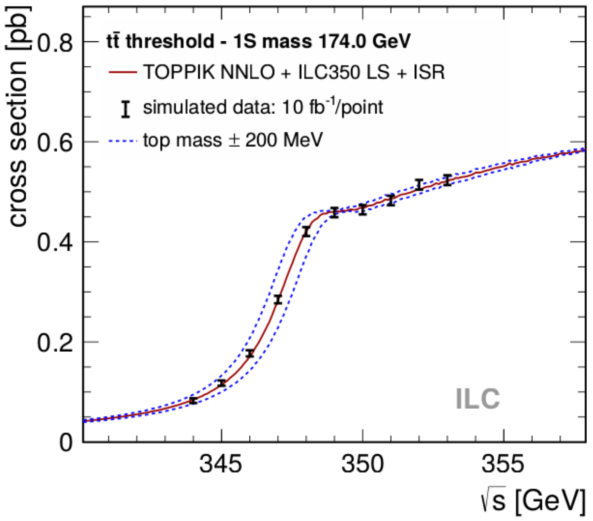
\includegraphics[width=0.5\textwidth]{Figures/Top_mass.pdf}
\caption[Top quark pair production cross section]{Top quark pair production cross section at the ILC350 after one year at the design luminosity~\cite[p. 15]{ILCPhysics}.}
\label{fig:Top_cross}
\end{figure}
\\At a center-of-mass energy of \SI{500}{\GeV}, further improvements in the precision measurements of the Higgs boson properties can be achieved.
As has been shown in Figure~\ref{fig:Higgs_couplings}, the Higgs coupling precisions will be reduced by a factor of two.
The Higgs coupling to the top can be derived from precision cross section measurements of $t\bar{t}H$ processes.
Since the top quark is the heaviest known elementary particle, it is expected to have the strongest coupling in the Higgs sector.
Therefore, its mass and its coupling to the Higgs boson are important quantities in many particle physics theories, and will be measured in a model independent manner as described in the section above.
The full ILC program will yield a precision of the Higgs coupling to the top quark of about \SI{2}{\percent} in model independent analyses~\cite{ttH_coupling}.
Only with such precisions, can deviations from Standard Model predictions be discovered, which has implications for new physics beyond the Standard Model.
Additionally, measuring the Higgs self-coupling in double Higgs production processes is another goal of the ILC500.
In the processes \positron +\electron$\rightarrow$ZHH and \positron +\electron$\rightarrow$ $\nu\bar{\nu}$HH (see Figure~\ref{fig:DoubleHiggsFeynman}), the Higgs self-coupling can be measured to a accuracy of \SI{16}{\percent} at the ILC stages at \SI{500}{\GeV} and \SI{1}{\TeV}~\cite{ttH_coupling}.
\begin{figure}
\centering
 \begin{minipage}[t]{0.55\textwidth}
\centering
\raisebox{0.5\height}{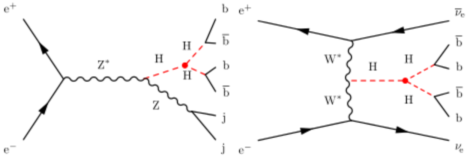
\includegraphics[width=\textwidth]{Figures/DoubleHiggs_Feynman.pdf}}
\caption[Feynman diagrams of double Higgs production processes]{Feynman diagrams of the processes \positron +\electron$\rightarrow$ZHH and \positron +\electron$\rightarrow$ $\nu\bar{\nu}$HH, with the subsequent decay of the Higgs boson to bottom quarks~\cite{ttH_coupling}.}
\label{fig:DoubleHiggsFeynman}
\end{minipage}
\hfill
\begin{minipage}[t]{0.44\textwidth}
\centering
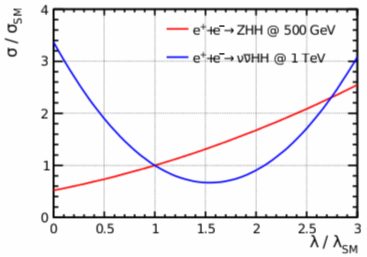
\includegraphics[width=\textwidth]{Figures/DoubleHiggs.pdf}
\caption[Double Higgs production cross sections]{Double Higgs production cross sections at the ILC normalized to the Standard Model cross section for different values of $\lambda$~\cite[p. 23]{ILC_Discovery}.}
\label{fig:DoubleHiggs}
\end{minipage}
\end{figure}
With these processes, the precision on the cross sections can indicate deviations from the Standard Model.
For higher and lower values for $\lambda$\footnote{$\lambda$ is a coefficient in the Higgs potential~\cite[p. 174]{PDG}.} compared to its Standard Model prediction, deviations from the Standard Model cross section can be observed, as shown in Figure~\ref{fig:DoubleHiggs}.
For the case that $\lambda = 2\lambda_{SM}$, the cross section for \positron + \electron $\rightarrow$ ZHH at the ILC500 is increased by about \SI{60}{\percent}.
\\In all stages, the discovery potential in precision measurements is considerably improved.
This includes searches for dark matter, supersymmetry (SUSY), and further beyond the Standard Model theories.
Figure~\ref{fig:MSSM_higgs_coupling} shows the predicted MSSM\footnote{The Minimal Supersymmetric Standard Model (MSSM) is a supersymmetry model that considers the minimum amount of particle states in addition to the Standard Model, in order to realize the SUSY phenomenology~\cite{MSSM}.} Higgs coupling deviations from Standard Model couplings.
For the bottom quark and the tau, the deviation is about \SI{3}{\percent}.
As shown in Figure~\ref{fig:Higgs_couplings} (b), the achievable HL-LHC coupling precision in these channels, however, ranges between 2 and \SI{7}{\percent}.
The aimed-for ILC precisions of between 0.5 and \SI{2}{\percent} for the coupling to the bottom quark and the tau will allow to distinguish the MSSM model from the Standard Model.
\begin{figure}
\centering
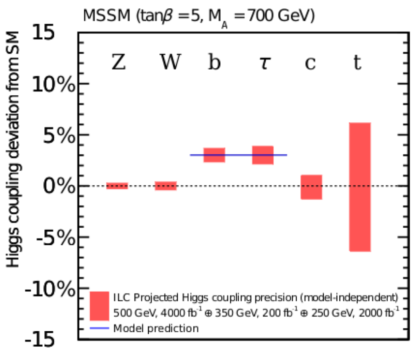
\includegraphics[width=0.45\textwidth]{Figures/MSSM_higgs_coupling.pdf}
\caption[Predicted MSSM deviations from SM Higgs couplings]{Predicted MSSM deviations from Standard Model Higgs couplings~\cite[p. 12]{ILCPhysics}.
The error bars represent the uncertainties expected from model independent analyses of the given ILC data set.}
\label{fig:MSSM_higgs_coupling}
\end{figure}
\\A complete overview of the physics motivation for the various ILC stages can be found in~\cite{PhysicsCase}.

\section{The experiments}
\label{ILC:detectors}
Previous sections have shown that the physics goals of the ILC are based on precision measurements that heavily rely on an outstanding detector performance in order to achieve the promised goals.
The performance requirements are accordingly strict, and the detectors are designed to fulfill them for the full energy range of operation.
Some of the requirements are: exceptional energy and spatial resolution, vertex recognition, and reliable flavor tagging.
Additionally, the detector designs have to address the background arising from beam-beam interactions and the accelerator itself, which is explained in Chapter~\ref{Backgrounds}.
Especially the forward detector systems have to be radiation hard to avoid radiation damage.
All these requirements are fulfilled in the design of the two ILC experiments.
\\In order to preserve competitive spirit and the ability to cross-check results, the ILC has two detectors despite the fact that it is a linear and not a circular collider.
The so-called push-pull system makes this possible by allowing the detectors to switch position after a certain amount of data-taking time.
The whole detector together with the last quadrupole magnet of the accelerator Final-Focus system will be pulled out of the beam line, and the other detector takes its place.
The whole process is designed to take from several hours up to 1-2 days, but involves some challenges especially for the magnets, the cryogenics, and the detector and machine alignment~\cite[p. 28-29]{TDR1}.
The two detectors, the Silicon Detector (\sid) and the International Large Detector (ILD), will be explained in detail in the following sections.
The focus will lie on \sid, since all the background studies presented in this thesis were done in the context of the \sid detector.

\subsection{The Silicon Detector}
\label{ILC:SiD}
The \sid is designed to be a robust, compact detector.
Its vertex and tracker system, as well as the electromagnetic calorimeter (ECAL) are purely based on silicon sensors.
The silicon design, in comparison to other designs for the vertex and tracking detectors, is more robust regarding the beam background and timing~\cite[cf. p. 57ff]{TDR4}.
\\Being designed to be compact, the measurements for the full detector are \SI{14}{m} in height and \SI{11}{m} in length.
To compensate the small radius, the magnetic field of the superconducting solenoid magnet is \SI{5}{T}, so that \sid is hermetic and contains the full particle showers.
The detector is optimized for Particle Flow Algorithms (PFA), in order to improve on the jet energy reconstruction capability.
PFA is a reconstruction method that reconstructs each particle of the final state individually and uses the different subdetectors for a specific purpose.
Therefore, charged particles are reconstructed from tracks in the tracker device.
The electromagnetic calorimeter (ECAL) is used for photons, and the electromagnetic (ECAL) and hadronic calorimeter (HCAL) together for other neutral particles~\cite{PFA}.
\\Table~\ref{tab:KeyParametersSiD} lists the key parameters and measurements of the \sid subdetector systems together with the technologies for the individual sub-systems.
Additionally, Figure~\ref{fig:SiD} shows a visualization of the \sid detector and its subdetectors, which will be explained in the following paragraphs.
A more detailed description can be found in~\cite{TDR4}.
\begin{figure}[h]
\centering
\includegraphics[width=0.8\textwidth]{Figures/SiD_new.jpg}
\caption[Visualization of the \sid detector]{The \sid detector consists of the vertex and tracking detectors (red), the electromagnetic calorimeter (ECAL) (green), the hadronic calorimeter (HCAL) (purple) and the muon system (gray).
All subdetectors except the muon system are inside the solenoid magnet.
Outside the muon endcaps is the detector specific background shielding, called ``Pacman'' with an inner (light gray) and an outer (beige) layer~\cite{SiD_Geo}.}
\label{fig:SiD}
\end{figure}

\begin{table}[h!]
\caption[Key parameters of the baseline \sid design]{Key parameters and technologies foreseen for the baseline \sid design. All dimensions are given in cm~\cite{SiD_Geo}.}
\label{tab:KeyParametersSiD}
\centering
\begin{tabularx}{0.81\textwidth}{l|llll}
\hline\hline
\sid Barrel & Technology & Inner radius & Outer radius & z extent\\
\hline
Vertex detector & Silicon pixels & 1.4 & 6.0 & $\pm 6.3$ \\
Tracker & Silicon strips & 21.5 & 121.5 & $\pm 150.3$ \\
ECAL & Silicon pixels-W & 126.5 & 140.3 & $\pm 176.5$ \\
HCAL & SiPM-steel & 140.3 & 256.8 & $\pm 295.0$ \\
Solenoid & 5 T SC & 260.4 & 342.9 & $\pm 295.0$ \\
Muon System & Scintillator-steel & 345.4 & 605.4 & $\pm 416.0$ \\
\hline
\sid Endcap & Technology & Inner z & Outer z & Outer radius\\
\hline
Vertex detector & Silicon pixels & 7.3 & 83.4 & 7.1 \\
Tracker & Silicon strips & 77.0 & 164.3 & 125.5 \\
ECAL & Silicon pixel-W & 165.7 & 180.0 & 126.5 \\
HCAL & SiPM-steel & 180.5 & 300.0 & 140.3 \\
Muon System & Scintillator/steel & 300.0 & 560.0 & 605.4 \\
LumiCal & Silicon-W & 155.7 & 169.55 &  20.0 \\
BeamCal & Semiconductor-W & 326.5 & 344 & 14.0 \\
\hline\hline
\end{tabularx}
\end{table}

\paragraph{Vertex detector}
The vertex detector, shown in Figure~\ref{fig:SiD_VXD}, will be the inner most subdetector with the measurements of a soda can.
With its five layers for the barrel and the endcaps, it will be able to do very precise measurements.
The requirements for the vertex detector performance are very demanding:
The spatial resolution with less than \SI{5}{\micro\meter} allows very precise tracking, whilst the impact parameter resolution is aimed for about \SI{3}{\micro\meter} for the verification of the primary vertex (see Figure~\ref{fig:vertex_res}), as well as of the secondary vertex of a bottom quark (b-tagging) and even of a charm quark (c-tagging).
The latter is very challenging due to the short flight distance of the charm quark of only a few microns before it hadronizes.
Figure~\ref{fig:tagging} shows the flavor tagging efficiency and the corresponding purity in di-jet samples.
Depending on the physics analysis, a working point can be chosen from the plot in order to find the correct balance between high statistics and low backgrounds.
\\Additionally, a very small material budget of about \SI{0.1}{\percent\xzero} per layer is foreseen for the vertex detector in order to limit particle showers and multiple scattering in this subdetector~\cite{SiD_Update,Marcels_general_SiD_slides}.
To achieve this minimal material budget, sensor technologies are considered that foresee the implementation of the sensor buffers on the chips directly to minimize the used material. 
For a comparison to the CMS pixel detector, Figure~\ref{fig:CMS} shows the material budget of the original and the upgraded detector.
The material budget is significantly reduced for the upgrade for $\eta$\footnote{$\eta$ is the pseudorapidity, which is commonly used in LHC experiments to express the angle relative to the beam axis: $\eta=-ln[tan(\theta/2)]$} above one.
In the high-$\eta$ ranges, the material budget reaches \SI{0.7}{\xzero}.
The \sid vertex detector material budget, which is shown in Figure~\ref{fig:SiD_material_budget}, reaches only \SI{0.04}{\xzero} up to the very forward regions. \todo{What are bumps in material budget? With which geometry was plot made?}
\\The final decision on the \sid sensor technology and the required pixel sizes is not made yet, which allows the detector to have the most recent state-of-the-art technology.
For simulation studies, a pixel size of \SI{20}{\micro\meter}$\times$\SI{20}{\micro\meter} is used.
The currently foreseen technology candidates are various designs based on silicon diode pixels, such as Monolithic Active Pixels (MAPS), Chronopix, Vertically Integrated (``3D'') chips, as well as High Voltage CMOS sensors~\cites[p. 70 ff]{TDR4}[p. 319 ff]{spieler}. 
\begin{figure}[h!]
\centering
\includegraphics[width=0.5\textwidth]{Figures/SiD_VXD_3D.png}
\caption[Visualization of the \sid vertex detector]{Visualization of the \sid vertex detector~\cite{SiD_Update2}.}
\label{fig:SiD_VXD}
\end{figure}

\begin{figure}[!h]
\centering
 \begin{minipage}[t]{0.44\textwidth}
 \centering
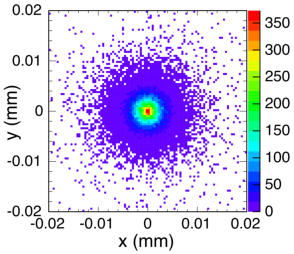
\includegraphics[width=0.95\textwidth]{Figures/Vertex_resolution.pdf}
\caption[\sid vertex resolution]{Positions of reconstructed primary vertices in simulated processes of the Z boson decaying to light quarks~\cite[p. 148]{TDR4}.}
\label{fig:vertex_res}
\end{minipage}
\hfill
\begin{minipage}[t]{0.55\textwidth}
\centering
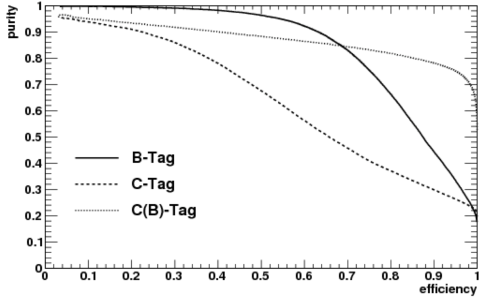
\includegraphics[width=\textwidth]{Figures/flavor_tagging_eff.pdf}
\caption[Flavor tagging efficiency in \sid]{Purity as a function of the flavor tagging efficiency in \sid for di-jet samples~\cite[p. 99]{LOI}.
The curves show the relation for b-tagging, c-tagging, and c-tagging with bottom quark background only.}
\label{fig:tagging}
\end{minipage}
\end{figure}

\begin{figure}[!h]
\centering
 \begin{minipage}[t]{0.49\textwidth}
 \centering
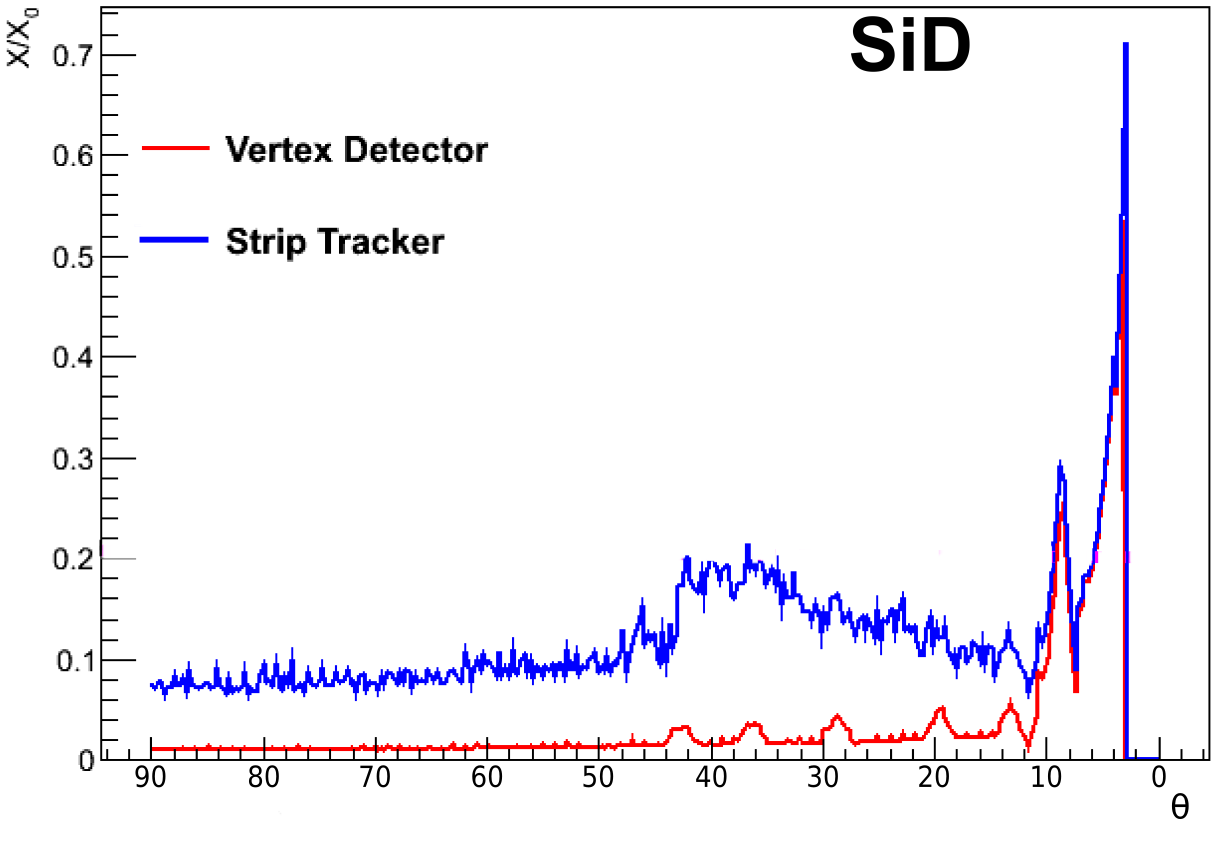
\includegraphics[width=\textwidth]{Figures/SiD_material_budget.png}
\caption[Material budget of the \sid vertex and tracker detector]{Material budget of the \sid vertex and tracker detector expressed in radiation lengths as a function of the angle to the beam axis~\cite[cf. p. 51]{Marcels_general_SiD_slides}.}
\label{fig:SiD_material_budget}
\end{minipage}
\hfill
\begin{minipage}[t]{0.49\textwidth}
\centering
\includegraphics[width=\textwidth]{Figures/CMS_Pixeldetector_materialbudget.png}
\caption[Material budget of the CMS pixel detector]{Material budget of the original and the upgraded CMS pixel detector expressed in radiation lengths as a function of $\eta$~\cite{CMS_pixeldetector}.}
\label{fig:CMS}
\end{minipage}
\end{figure}


\begin{figure}[h!]
\centering
\includegraphics[width=0.5\textwidth]{Figures/SiD_Tracker.png}
\caption[Drawing of the \sid tracking detector]{The \sid tracking detector layout~\cite{SiD_Update2}.
The drawing includes the vertex detector in the center.}
\label{fig:SiD_tracker}
\end{figure}

\paragraph{Tracking detector}
Outside the vertex detector is the Silicon Tracker, which can be seen in Figure~\ref{fig:SiD_tracker}.
For its five barrel layers and four endcap layers, \num{0.05}$\times$\SI{100}{\milli\meter\squared} sized silicon strip sensors are planned that will use so-called KPiX ASIC readout chips.
These KPiX chips have a buffer depth of four in the current design, which means that up to four hits per sensor can be stored on the chip's buffer.
Any further hit can not be recorded and is lost, which is explained again in more detail below.
That makes thorough simulations of the expected backgrounds reaching the detector very important.
The sensors can still be adapted with respect to design and technology used, so that the detector will be optimized as best as possible.

\paragraph{Calorimeters}
The electromagnetic calorimeter (ECAL) will be using KPiX chips as well, as it is also based on silicon sensors.
The ECAL with its 30 layers is designed to be a granular imaging calorimeter with a pixel size of \SI{3.5}{\milli\meter}$\times$\SI{3.5}{\milli\meter}, meaning that electromagnetic particle showers developing in the tungsten layers between the sensitive silicon layers can not only be measured in width and length, but rather their shower particles can be tracked individually.
\\The same will be true for the highly segmented hadronic calorimeter (HCAL) with a pixel size of \SI{1}{\centi\meter}$\times$\SI{1}{\centi\meter}.
With all subdetectors mentioned so far being inside the \SI{5}{\tesla} solenoid field of the \sid solenoid magnet, particle tracking is therefore possible not only in the tracking subdetectors, but even in the calorimeters.
The 40 active layers of the HCAL will contain scintillators and silicon photomultipliers (SiPM) measuring particle showers that are developing in the steel layers in between.
\begin{figure}[h!]
\centering
\includegraphics[width=0.5\textwidth]{Figures/SiD_PFA.png}
\caption[Visualization of the granulat \sid subdetectors]{Simulation of a physics event in the \sid detector~\cite{SiD_Update2}.
The particle showers, which start to develop in the ECAL, are easily distinguishable thanks to the highly granular calorimeters.}
\label{fig:SiD_PFA}
\end{figure}

\paragraph{Muon system}
The muon chamber, which is the only subdetector outside the solenoid magnet, will use long scintillator strips with SiPM readout based on the HCAL sensor technology.
Its purpose is not only to identify muons being produced in the beam collisions, but also to record the tail of hadronic showers that have started in the HCAL.

\paragraph{Forward system}
The forward systems of \sid make the detector hermetic, i.e. the detector is a closed system which can catch particles under almost all solid angles.
The forward region covers a polar angle $\theta > $ \SI{3}{\milli\radian}.
Boosted particles with high momentum along the beam direction that go under an angle $\theta < $ \SI{3}{\milli\radian} will therefore escape the detector.
These losses are unavoidable since detector components cannot be built inside the beam pipe and the detector is not designed for physics that require measurements of these small-angle particles.
The forward system consists of the Luminosity Calorimeter (LumiCal) and the Beam Calorimeter (BeamCal).
Apart from making \sid hermetic, the LumiCal will measure the luminosity integrated over time, whilst the BeamCal will give an indication of the instantaneous luminosity by measuring the \positron \electron pair background from beam-beam interactions, which is explained in Section~\ref{BeamBeam:pairs}.
Since the pair background is directly dependent on the beam qualities, the BeamCal measurements will indicate variations in the beam parameters.
Like the ECAL, both, the LumiCal and the BeamCal, are sampling calorimeters using tungsten layers for the particle shower development and semiconductors for the sensitive layers.
As the forward region is highly affected by high-energy particles that are typically boosted in the forward direction, the sensors have to be specifically designed to withstand radiation damage.
The damage results from large energy depositions from the boosted particles as well as from different backgrounds, such as the pair background as mentioned before.
With this flux of particles hitting the forward system, the BeamCal is expected to have an occupancy of \SI{100}{\percent}, i.e. all of the BeamCal pixels are expected to be hit by particles.
This large occupancy is accounted for in the readout technology~\cite[p. 133ff]{TDR4}.
\begin{figure}[h!]
\centering
\includegraphics[width=0.7\textwidth]{Figures/SiD_Forward.png}
\caption[Drawing of the \sid forward detectors]{Layout drawing of the \sid forward detectors~\cite[p. 134]{TDR4}.
All dimensions are given in mm.}
\label{fig:SiD_Forward}
\end{figure}

\paragraph{Pacman}
Part of the detector, but not part of the sensitive subdetectors, is ``Pacman''.
Pacman is a detector specific shielding against machine background that reaches the detector and would increase the detector occupancy.
All particles that are produced from the beam interacting with accelerator machine parts, and that reach the detectors, are called machine background.
The Pacman shielding is placed on either side of the detector, and has an outer radius of about \SI{2.8}{\meter}, hence it covers the full radius of all subdetectors inside the solenoid magnet.
The inner layer of Pacman is made of iron, the outer layer of boronated concrete which is specially designed to stop neutrons.
The thickness is about \SI{3.4}{\meter}~\cite{SiD_Geo}.
Its use can be seen in the simulation of the machine backgrounds in Chapters~\ref{BDS_Muons:SiD} and \ref{BeamDumps:SiDocc}.

\paragraph{Detector readout architecture}
As mentioned above, the readout architecture for the \sid detector foresees a buffer depth of four in the current design.
The number of available buffers is an important issue for the performance of the detector, and is therefore topic of the \sid simulation studies with respect to the background occupancies.
As explained in Section~\ref{PairBkg:occupancy} in more detail, the detector occupancy is the fraction of hits per detector cell, which is calculated by counting the hits in the individual cells.
If the number of hits per cell exceeds the number of available buffers (the buffer depth), the cell cannot store any further hits.
A refined detector optimization is therefore crucial with respect to the occurring background rates.
\\Table~\ref{tab:ILC_parameters} lists the ILC beam parameters in the different ILC stages.
The ILC will deliver beam trains, which contain 1312 beam bunches in the first stage, at a rate of \SI{5}{\hertz}.
Each of the bunches is separated by \SI{554}{\nano\second}, resulting in a total train duration of \SI{0.72}{\milli\second}.
The time gap of \SI{199}{\milli\second} between successive trains is used for reading out the analog signals of the detector buffers, and for their digital processing.
The motivation of the ILC experiment is to record all measured events without rejecting any of them by the use of triggers, as explained in Section~\ref{ILC:physicsmotivation}.
\\Due to this, the detector background occupancy has to be below a critical acceptance limit.
For the optimization of the detector readout design and its buffer depth, detailed occupancy studies are needed.
In all of the background simulation studies presented in the following chapters, the \sid occupancy has been evaluated with respect to the critical acceptance limit.

\paragraph{\sid detector variants}
Since the publication of the Technical Design Report about the design details of the ILC accelerator, the detectors, and the facilities, there have been official changes to the design.
The changes regarding the overall accelerator and facility design are suggested as Change Requests (CR), and are reviewed and approved by a Technical Change and Management Board~\cite{TCMB}. 
Some of the Change Requests affect the detector designs directly, such as the change of L*, the distance between the interaction point (IP) and the last quadrupole magnet (QD0) of the Final-Focus system.
But there are also changes to the detector concepts, that are made internally by the detector groups.\\
There are major \sid detector design variants that are subject of discussions and simulation studies:
\begin{itemize}
 \item \underline{Change of L*}\\
 As the focal length of the last quadrupole magnet (QD0) of the Final-Focus system, which focuses the beam onto the IP, is smaller than the detector length, both detector concepts have their own QD0 magnets.
 These magnets are part of the detector's push-pull system.
 The official Change Request CR-002~\cite{CR-002} decided on a common L* for both detector concepts.
 Before, the distance (L*) between the IP and QD0 was different for \sid and ILD, as L* is dependent on the size of the detector.
 Since the diverging L* values mean different beam operation conditions, CR-002 dictated a change of the detector designs in such a way that L* is the same for both detectors, in order to facilitate the beam operation.
 For \sid, the dictated change of L* from 3.5 to \SI{4.1}{\meter} implied in practice that the BeamCal had to be repositioned, since it is attached to the QD0 support structure. 
 The BeamCal moved from a former distance to the IP of 2.95 to \SI{3.265}{\meter}~\cite{SiDBkgNote}.
 \item \underline{Design variants of the inner region of the BeamCal}\\
 The BeamCal surrounds the ingoing and outgoing beam pipe.
 For the inner region around the beam pipes, there are three different design variants that include a different amount of instrumentation, as shown in Figure~\ref{fig:BeamCal}.
 By cutting out the area between the beam pipes, the sensitive material is removed from the inner region with the highest density of background flux.
 Doing so will reduce the overall BeamCal radiation damage, but also lessens the potential for measuring physics events in that region.
 \begin{figure}
 \centering
  \begin{subfigure}[b]{0.3\textwidth}
   \centering
    \includegraphics[width=0.6\textwidth]{Figures/beamcal_plug.png}
   \caption{Instrumented inner region}
  \end{subfigure}
  \begin{subfigure}[b]{0.3\textwidth}
   \centering
    \includegraphics[width=0.6\textwidth]{Figures/beamcal_wedge.png}
   \caption{Wedge cutout}
   \end{subfigure}
    \begin{subfigure}[b]{0.3\textwidth}
   \centering
    \includegraphics[width=0.6\textwidth]{Figures/beamcal_circle.png}
   \caption{Circle cutout}
   \end{subfigure}
   \caption[Design variants of the \sid BeamCal]{Three different design variants of the inner region of the \sid BeamCal.
   From (a) to (c), the instrumentation of the inner region decreases with an increasing fraction of material cut out.}
   \label{fig:BeamCal}
 \end{figure}
 \item \underline{Anti-DiD Field}\\
 The BeamCal is expected to have an occupancy of \SI{100}{\percent} due to boosted particles as well as background particles such as the \positron\electron pairs from beam-beam interactions, as explained before.
 In order to suppress hits from these \positron\electron pairs, it was proposed to include an additional magnet in the detector design, the so-called anti-DiD (Detector Integrated Dipole) magnet~\cite{antiDiD}.
 The dipole windings of the anti-DiD are directly mounted around the \sid solenoid magnet.
 Its magnetic field has a value of \SI{600}{\gauss}, and causes locally the deflection of the pair background in the region of the BeamCal~\cite[p. 118]{TDR4}.
 The pairs are swept into the outgoing beam pipe, which reduces the BeamCal occupancy.
\end{itemize}

\subsection{The International Large Detector} 
\begin{figure}[h]
\centering
\includegraphics[width=0.7\textwidth]{Figures/ILD.png}
\caption[Schematic drawing of the ILD detector]{The ILD detector consists of the vertex detector (pink), the time projection chamber (TPC) (yellow), the electromagnetic calorimeter (ECAL) (blue), the hadronic calorimeter (HCAL) (green) and the muon system (gray). All subdetectors except the muon system are inside the solenoid magnet.\cite[p. 34]{TDR1}}
\label{fig:ILD}
\end{figure}
Like the \sid detector, ILD is a multi-purpose particle detector that is optimized for PFA.
Its vertex detector is also based on silicon sensors, whereas the tracker is a combination of both, a silicon strip and pixel detector, and a time projection chamber (TPC).
Also similar to \sid, the calorimeters are within the solenoid magnet, which is surrounded only by the muon system.
The magnetic field of the superconducting solenoid magnet is \SI{3.5}{T}.
Because of having a big gaseous volume, the full detector is bigger than \sid, namely \SI{16}{m} in height and \SI{14}{m} in length.
Figure~\ref{fig:ILD} shows all the subdetectors mentioned above in two schematics of the ILD detector.
